\documentclass[11pt,a4paper]{article}
\usepackage[margin=22mm,headheight=16pt,footskip=12mm]{geometry}
\usepackage[T1]{fontenc}
\usepackage[utf8]{inputenc}
\usepackage{lmodern,amsmath,amssymb,graphicx,xcolor,booktabs,longtable,array,tabularx}
\usepackage{tikz,float,caption,fancyhdr,titlesec,url,lscape}
\usetikzlibrary{arrows.meta,positioning,calc}
\definecolor{navy}{HTML}{16324F}
\definecolor{teal}{HTML}{007F86}
\definecolor{pale}{HTML}{EAF5F5}
\definecolor{ink}{HTML}{243646}
\definecolor{amber}{HTML}{A45C13}
\pdfinfo{/Title (Inverse-GPR Virtual-Fuel PI Controller) /Author (T-MATS Controller Development Study)}
\urlstyle{tt}
\setlength{\parindent}{0pt}
\setlength{\parskip}{5pt plus 1pt minus 1pt}
\setlength{\emergencystretch}{2em}
\widowpenalty=10000\clubpenalty=10000
\linespread{1.05}
\titleformat{\section}{\Large\sffamily\bfseries\color{navy}}{\thesection}{.7em}{}
\titleformat{\subsection}{\large\sffamily\bfseries\color{teal}}{\thesubsection}{.7em}{}
\titlespacing*{\section}{0pt}{19pt}{8pt}
\titlespacing*{\subsection}{0pt}{13pt}{5pt}
\captionsetup{font=small,labelfont={bf,color=navy},skip=8pt}
\pagestyle{fancy}\fancyhf{}
\fancyhead[L]{\small\sffamily\color{navy}POLY2 PID / 9250 RPM RETUNING}
\fancyhead[R]{\small\sffamily T-MATS control study}
\fancyfoot[L]{\scriptsize\color{ink}Sea level ISA 0 / fixed polynomial model}
\fancyfoot[R]{\small\thepage}
\renewcommand{\headrulewidth}{.3pt}
\tikzset{block/.style={draw=navy!55,fill=navy!3,rounded corners=3pt,minimum height=.92cm,align=center,font=\sffamily\small,inner sep=5pt},
gp/.style={block,draw=teal,fill=pale},plant/.style={block,draw=navy,fill=navy!12},
sum/.style={circle,draw=navy,minimum size=.68cm,fill=white,font=\large},
arr/.style={-{Latex[length=2.2mm]},draw=navy,line width=.65pt},
lab/.style={font=\small,fill=white,inner sep=2pt},
note/.style={font=\small\sffamily,text=ink,align=left}}
\begin{document}
\begin{titlepage}\color{navy}\sffamily
{\small T-MATS / POLY2 PID / OPERATING-POINT RETUNING}\par\vspace{22mm}
{\fontsize{30}{36}\selectfont\bfseries Retuning Poly2 PID\\at 9250 rpm, Sea Level, ISA 0\par}
\vspace{12mm}{\Large Joint tracking and fuel-ringing objective\par}
\vspace{10mm}\color{teal}\rule{\linewidth}{1.2pt}\color{navy}\vspace{8mm}
\begin{tabular}{ll}
Inverse & Frozen full-quadratic, four-input fuel model\\[5pt]
Feedforward & Same static $p_2(r,0,T,P)$ term\\[5pt]
Tuning condition & 9250 rpm, 0 m, ISA 0, Mach 0\\[5pt]
Tuning excitation & 10\% shaft-load application/removal pulses\\[5pt]
Validation & 5\% load pulses, evaluated after selection\\[5pt]
Preparation / evaluation & 60 s / 90 s
\end{tabular}
\par\vspace{12mm}\normalfont\color{ink}
The polynomial model, controller architecture, sensor, acceleration filter and actuator command limits are preserved. Only the three PID coefficients are retuned. The disturbance protocol follows the earlier fixed-speed study because the requested new condition specifies an operating point rather than a speed-ramp cycle.
\vfill The requested speed lies slightly below the original training-speed minimum. The model is not refitted, and this extrapolation is reported explicitly.
\end{titlepage}
\section{Selected gains and test definition}
\begin{table}[H]\centering\small\begin{tabular}{lrrr}\toprule
Controller & $K_p$ & $K_i$ & $K_d$\\\midrule
Base PI & 0.025 & 0.05 & 0\\
Original Poly2 & 0.025 & 0.1 & 0.002\\
Retuned Poly2 & 0.025 & 0.14 & 0.00125\\
\bottomrule\end{tabular}\caption{The derivative coefficient multiplies the normalized, filtered acceleration feedback, as in the original R3 architecture.}\end{table}
The unchanged R3-style Poly2 controller is
\begin{align}
\tilde e_N&=\frac{p_2(r,0,T,P)-p_2(N_s,0,T,P)}{\partial_N p_2(r,0,T,P)},\\
\tilde a&=\frac{p_2(N_s,\hat a,T,P)-p_2(N_s,0,T,P)}{\partial_a p_2(r,0,T,P)},\\
u^*&=p_2(r,0,T,P)+K_p\tilde e_N-K_d\tilde a+I,\qquad \dot I=K_i\tilde e_N.
\end{align}
The existing guards substitute speed error and filtered acceleration if inverse slopes, error ratios or the compressor map coordinate are unsuitable. The 0.03 s acceleration filter, 0.015 s sampling, fuel limits and conditional integration remain unchanged. The previous gains were $[0.025,0.1,0.002]$.

An unloaded trim establishes condition-specific turbine shaft power before any controller comparison. Ten percent of this reference is then applied at evaluation times 10.005, 30 and 60 s and removed at 15, 40.005 and 75 s. The load reference is 15376.792 hp, so the tuning pulses are 1537.6792 hp. All cases use the same load and 9250 rpm request; no ambient variation is added.
\section{Selection objective and search}
For each numerically accepted candidate, minimize
\begin{equation}
J=\max\left(\frac{\mathrm{RMSE}}{\mathrm{RMSE}_{\rm original}},\frac{R}{R_{\rm original}}\right).
\end{equation}
The denominator is the original Poly2 controller at the same condition. The base PI is a comparator, not part of the candidate selection. The initial sweep includes the original gains and a $3\times3\times3$ grid with $K_p\in\{0.015,0.025,0.035\}$, $K_i\in\{0.08,0.14,0.20\}$ and $K_d\in\{0.001,0.002,0.003\}$. A local refinement changes each coefficient of the best grid point separately by $\pm25\%$.

All 34 Poly2 candidates are retained. Candidate 34 is the best tested under this declared objective; this is a bounded search, not a proof of a global optimum. Gains are frozen before the 5\% validation case.
\clearpage
\section{Tuning-condition results}
\begin{table}[H]\centering\small\begin{tabular}{lrrr}\toprule
Metric & Base PI & Original Poly2 & Retuned Poly2\\\midrule
Speed RMSE (rpm) & 2.421 & 1.666 & 1.546\\
Peak speed error (rpm) & 21.41 & 14.11 & 15.82\\
IAE (rpm s) & 51.12 & 28.53 & 21.66\\
Fuel ringing (lbm/s) & 2.07 & 1.697 & 1.299\\
Recovery to 1 percent (s) & 0 & 0 & 0\\
Recovery to 0.1 rpm (s) & 2.475 & 1.365 & 0.93\\
Minimum surge margin (percent) & 18.28 & 19.63 & 18.94\\
Peak fuel (lbm/s) & 1.956 & 1.888 & 1.925\\
Maximum fuel slew (lbm/s squared) & 4.817 & 8.719 & 7.274\\
Fuel saturation (percent) & 0 & 0 & 0\\
\bottomrule\end{tabular}\caption{10 percent shaft-load pulses at the requested condition. Recovery is the worst of six application/removal events; NR means no persistent entry before the next edge.}\end{table}
Relative to the original Poly2 controller, the selected gains give: RMSE: -7.2\% ringing: -23.4\% peak error: +12.1\%.

The selected setting leaves proportional action unchanged, raises integral gain by 40\% and reduces derivative gain by 37.5\%. It gives faster fine settling and less cumulative fuel reversal, but the peak speed excursion is larger than with the original Poly2 setting. This tradeoff is consistent with reduced acceleration feedback allowing a larger initial departure, while stronger integral action removes the remaining error sooner. The measured trace, rather than this interpretation alone, establishes the performance change. The objective explicitly balances RMSE and ringing; it does not minimize peak error or establish robustness away from this operating point.

Speed RMSE is measured over the complete 90 s evaluation. Ringing is the sum of fuel total variation minus net fuel change in six two-second load-edge windows. It is measured in lbm/s, not total fuel consumption. The broad 1\% band is $\pm92.5$ rpm; zero recovery means no band exit. The 0.1 rpm criterion exposes finer settling and requires persistent entry through the end of each event interval.
\begin{figure}[H]\centering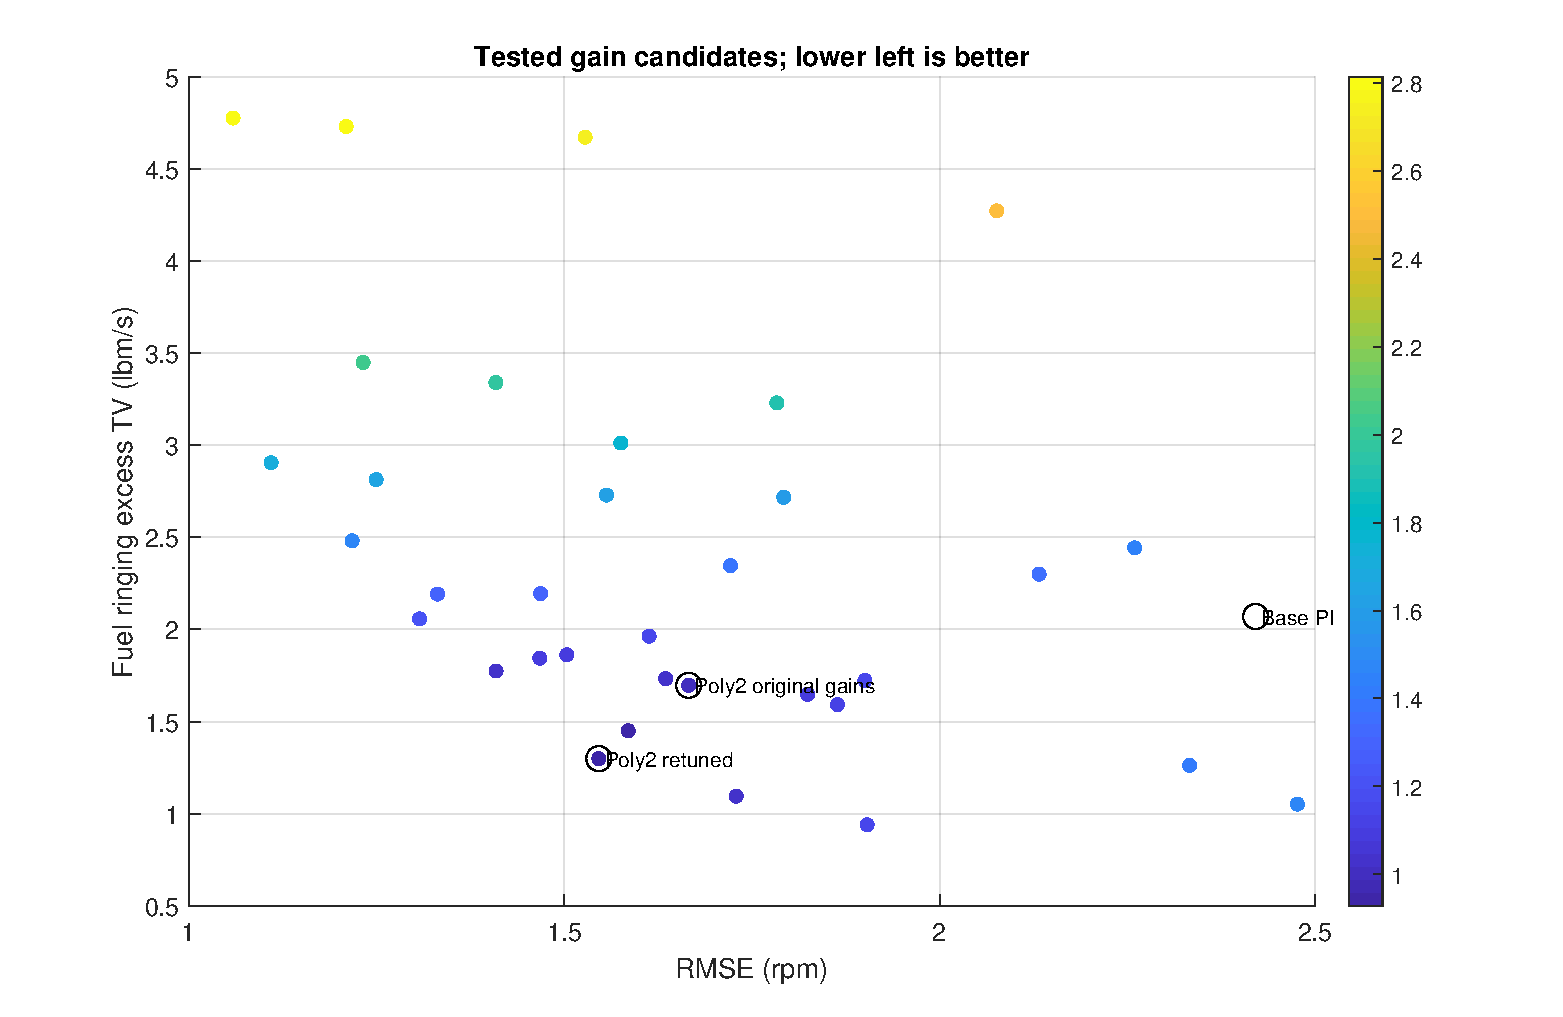
\includegraphics[width=\linewidth]{poly9250_tuning.pdf}\caption{All accepted Poly2 candidates, coloured by the joint objective; original and selected gains and base PI are identified.}\end{figure}
\clearpage
\section{Full and zoomed time-domain responses}
\begin{figure}[H]\centering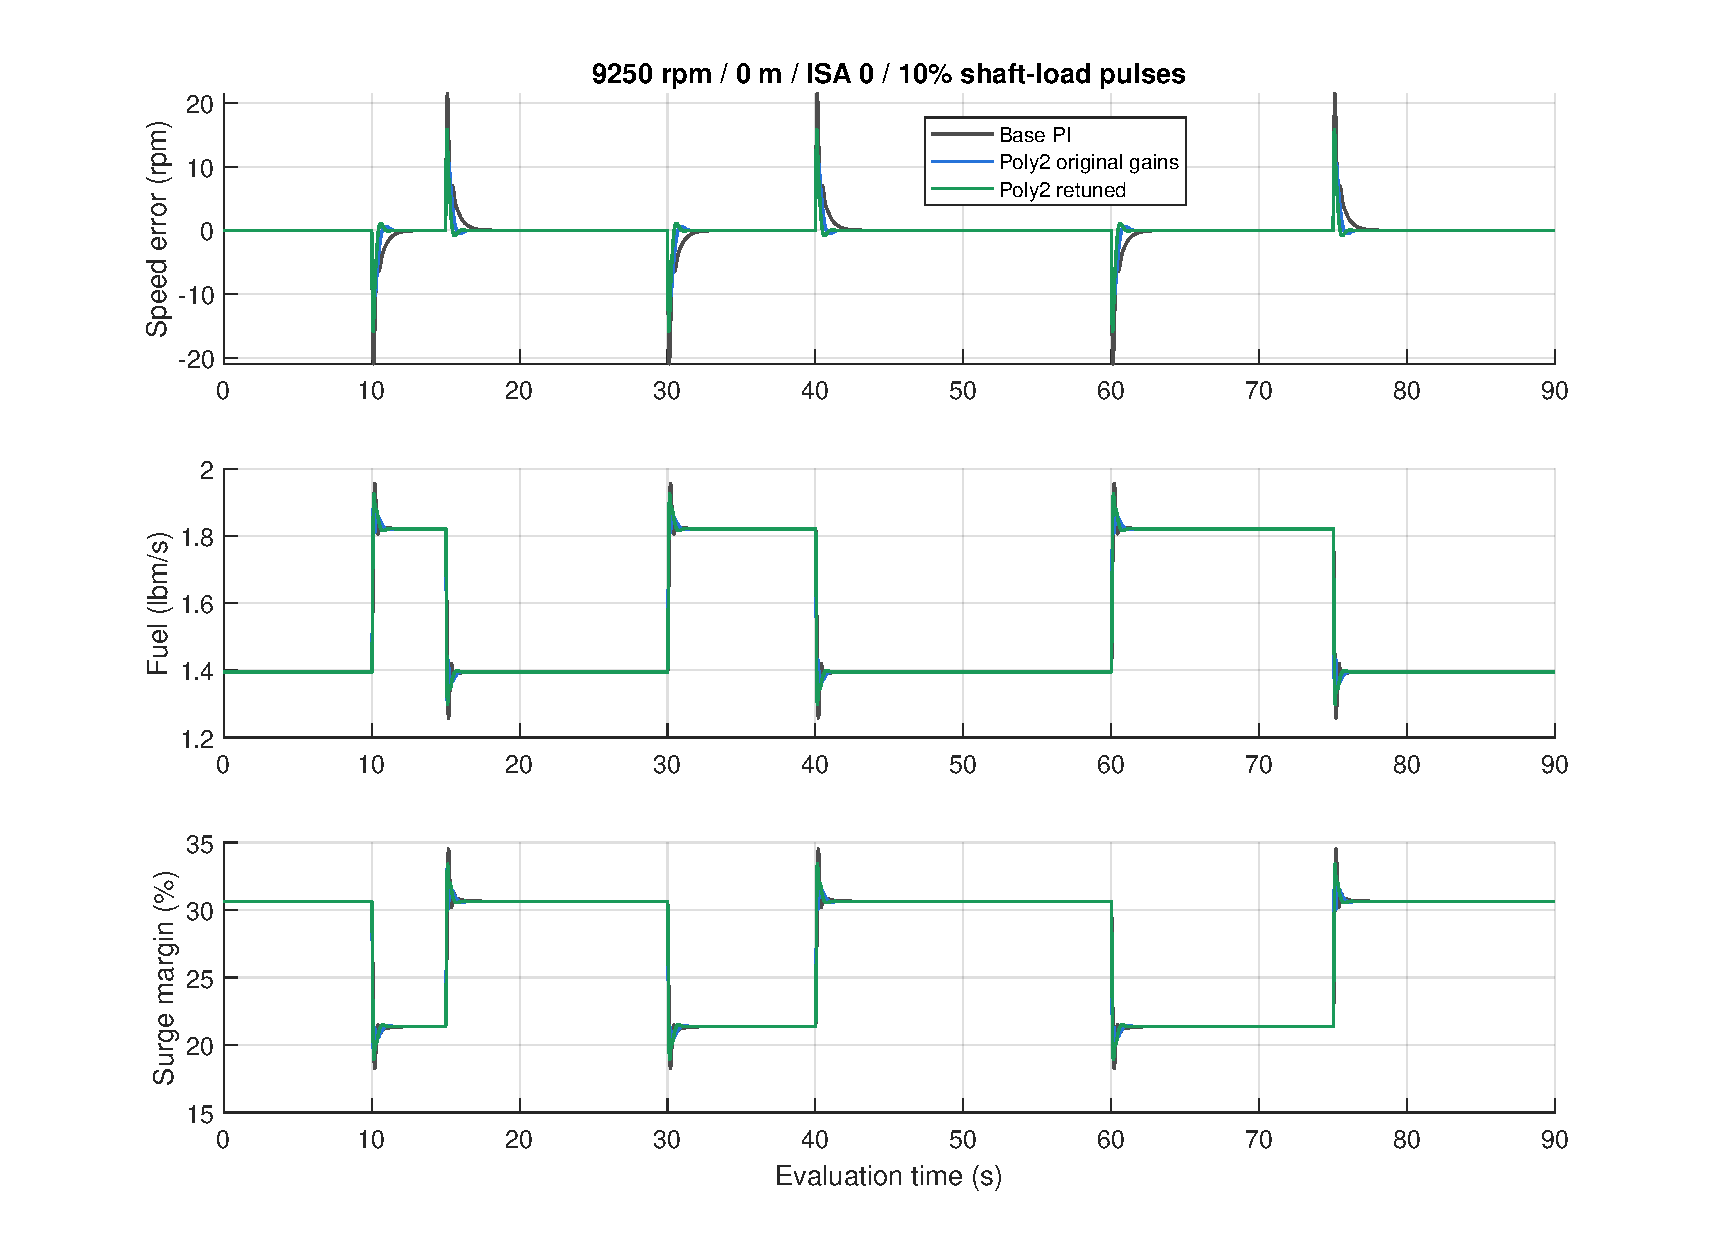
\includegraphics[width=\linewidth]{poly9250_overview.pdf}\caption{Identical 10 percent shaft-load pulses with base PI, original Poly2 and selected Poly2 gains.}\end{figure}
\clearpage
\begin{figure}[H]\centering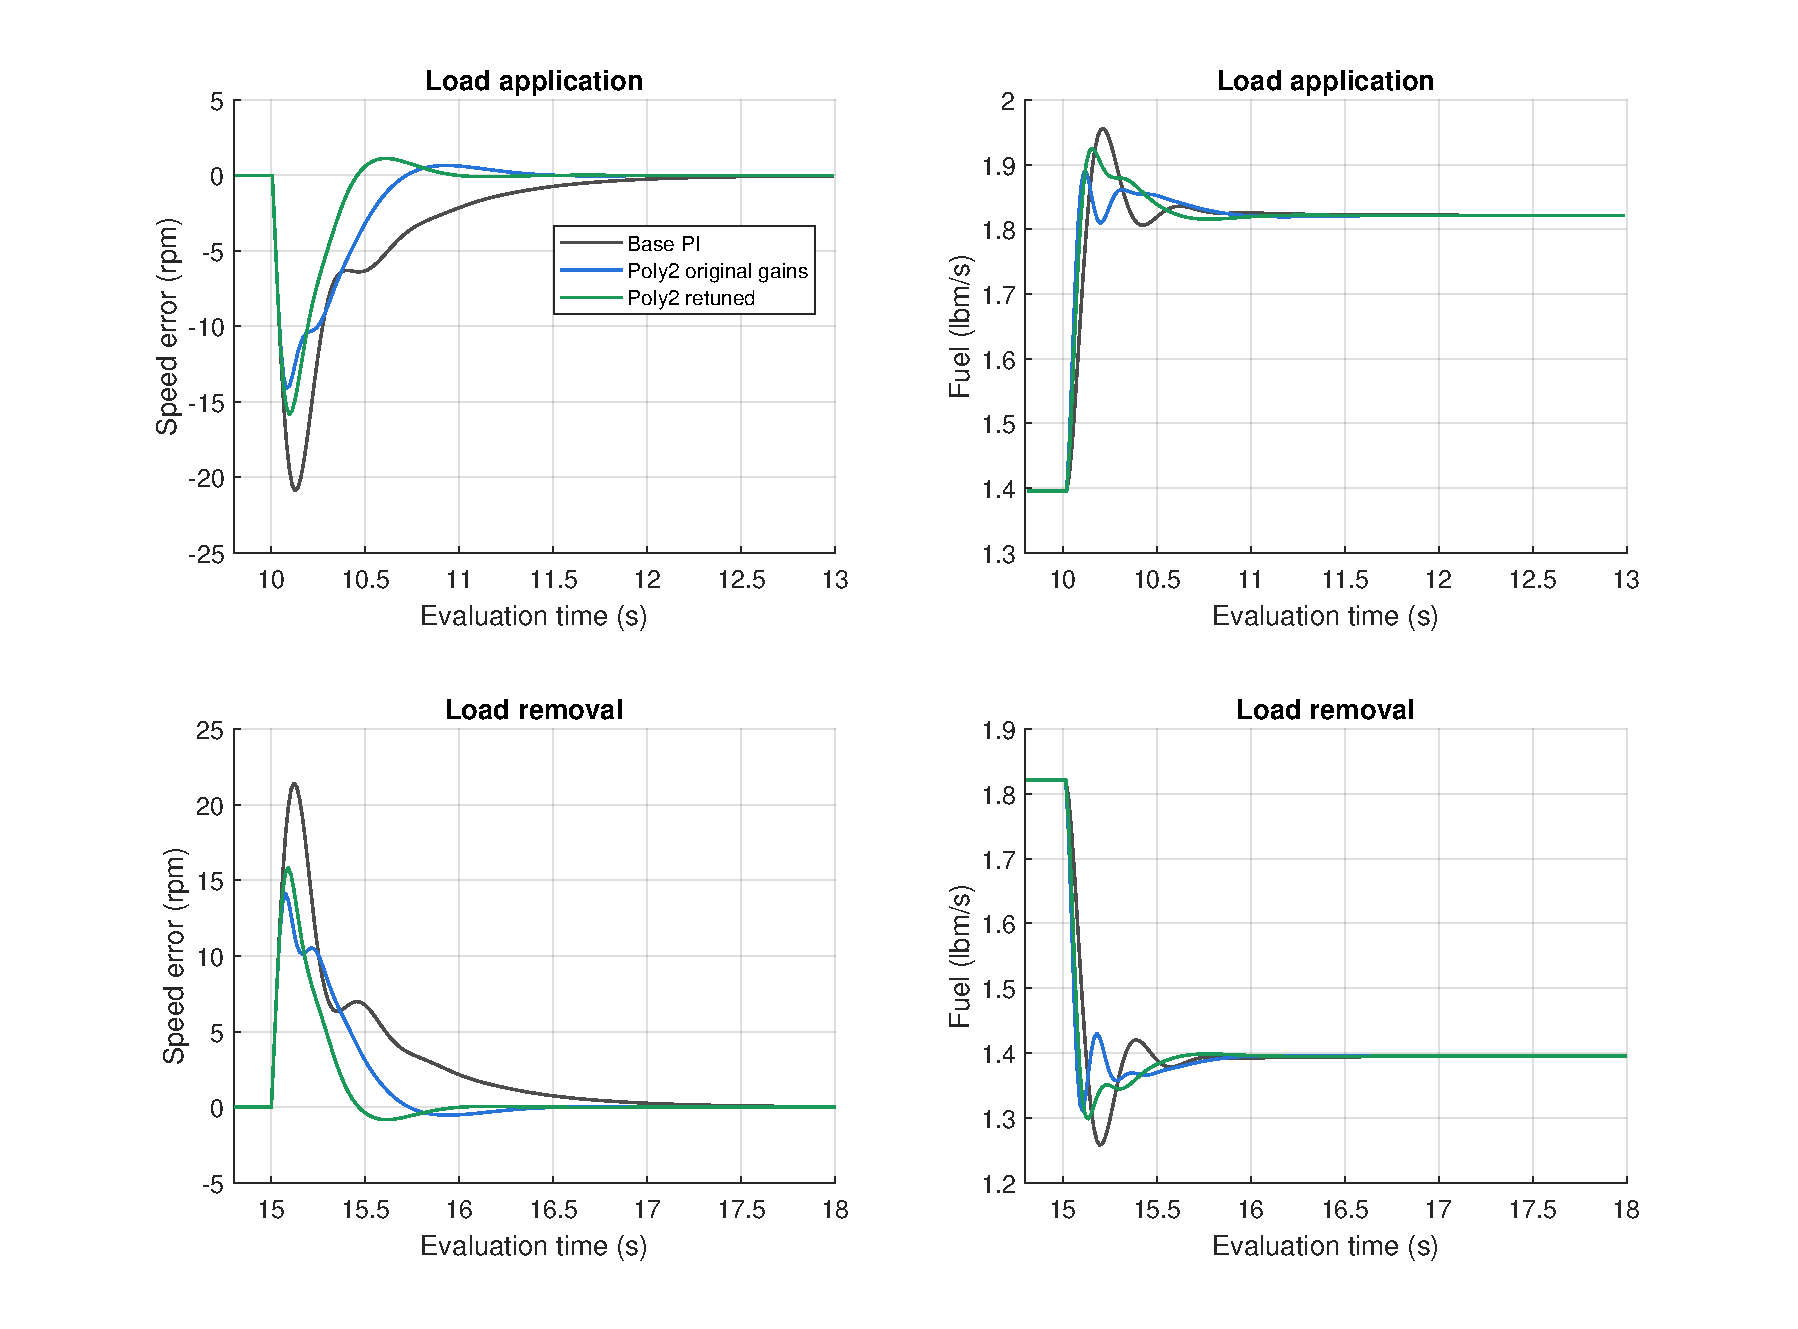
\includegraphics[width=\linewidth]{poly9250_zoom.pdf}\caption{First load application and removal, including speed error and fuel-command reversals.}\end{figure}
\clearpage
\section{Frozen-gain 5 percent validation}
\begin{table}[H]\centering\small\begin{tabular}{lrrr}\toprule
Metric & Base PI & Original Poly2 & Retuned Poly2\\\midrule
Speed RMSE (rpm) & 1.169 & 0.8018 & 0.7439\\
Peak speed error (rpm) & 10.39 & 6.969 & 7.806\\
IAE (rpm s) & 24.63 & 13.64 & 10.27\\
Fuel ringing (lbm/s) & 1.058 & 0.9005 & 0.6544\\
Recovery to 1 percent (s) & 0 & 0 & 0\\
Recovery to 0.1 rpm (s) & 2.115 & 1.26 & 0.87\\
\bottomrule\end{tabular}\caption{Independent 5 percent load-amplitude check after gain selection. These results are not used to select or refine gains.}\end{table}
The validation halves the disturbance magnitude and preserves timing, model, environment and selected gains. It tests amplitude transfer at this operating point; it is not validation at another speed or altitude. No subsequent gain selection is based on these results.
\section{Coverage, validity and reproduction}
The original training-speed interval is approximately 9264.23--9750.60 rpm. The requested 9250 rpm setpoint is 14.23 rpm below it, and disturbances can move actual speed farther below. Consequently the static inverse query is outside the fitted speed interval throughout evaluation. This repeat intentionally honors the requested condition rather than silently shifting it into the old covered envelope. Numerical convergence does not turn extrapolation into in-domain model validation.

The accepted runs satisfy finite valid plant signals, positive fuel and surge margin, converged flow residuals, solver iteration limits, a settled pre-test speed and full duration. Saved controller commands and integral updates are independently replayed, and the RMSE and ringing metrics are recomputed from traces. Fallback and map diagnostics are retained with each run.

Open \path{GasTurbine_Poly2_9250_Tuned.mdl} in the existing T-MATS workspace. Its preload callback \path{tmats_poly9250_tuned_setup.m} loads the selected gains and unchanged polynomial. The search runner is \path{run_tmats_poly9250.m}; selection is \path{select_tmats_poly9250.m}; amplitude validation is \path{validate_tmats_poly9250.m}. All trials, selected parameters, native traces and validation results are under \path{results/poly2_tune9250_20260915}. Original controller files and fitted coefficients are preserved.
\end{document}
